\documentclass[a4paper,12pt]{article}
\usepackage[utf8]{inputenc}
\usepackage[german]{babel}
\usepackage{amsmath}
\usepackage{amssymb}
\usepackage{amsthm}
\usepackage{geometry}
\usepackage{graphicx}
\usepackage[hidelinks]{hyperref}
\usepackage{listings}
\usepackage{xcolor}
\usepackage{enumitem}
\usepackage{booktabs}
\usepackage{array}
\usepackage{multirow}

\geometry{margin=2.5cm}

\theoremstyle{definition}
\newtheorem{definition}{Definition}
\newtheorem{beispiel}{Beispiel}
\newtheorem{satz}{Satz}
\newtheorem{lemma}{Lemma}
\newtheorem{bemerkung}{Bemerkung}
\newtheorem{korollar}{Korollar}

\setlist[itemize,1]{label=--}

% ---------- Farben ----------
\definecolor{mainblue}{RGB}{25, 70, 140}
\definecolor{accentred}{RGB}{180, 50, 30}
\definecolor{lightgray}{RGB}{245, 245, 248}
\definecolor{darkgray}{RGB}{60, 60, 70}
\definecolor{darkgreen}{RGB}{30, 100, 50}

\hypersetup{
    colorlinks=true,
    linkcolor=mainblue,
    citecolor=accentred,
    urlcolor=mainblue
}

\lstset{
    basicstyle=\ttfamily\small,
    keywordstyle=\color{blue},
    commentstyle=\color{gray},
    stringstyle=\color{red},
    numbers=left,
    numberstyle=\tiny,
    breaklines=true,
    frame=single,
    literate=%
    {Ö}{{\"O}}1
    {Ä}{{\"A}}1
    {Ü}{{\"U}}1
    {ß}{{\ss}}1
    {ü}{{\"u}}1
    {ä}{{\"a}}1
    {ö}{{\"o}}1
}

\title{\textbf{Formale Analyse eines Mobilfunknetz-basierten\\
Drohnenabwehrsystems mittels des Subgraph Algorithmus}\\[0.5em]
\large Graphentheoretische Modellierung und algorithmische Verifikation\\
eines nationalen Drohnen-Abwehrschirms}
\author{Stephan Epp\\[0.3em]
\small Universit\"at Bielefeld}
\date{12. Mai 2026}

\begin{document}

\maketitle

\begin{abstract}
Die vorliegende Arbeit entwickelt ein formales Rahmenwerk zur Analyse und Verifikation
eines Mobilfunknetz-basierten Drohnenabwehrsystems, wie es von der Deutschen Telekom
und Rheinmetall f\"ur den Schutz kritischer Infrastrukturen in Deutschland angestrebt wird.
Das Kernelement der Analyse ist der \emph{Subgraph Algorithmus} (Epp 2026) mit
Laufzeitkomplexit\"at $\Theta(n^3)$, der auf die graphentheoretische Repr\"asentation
des Mobilfunknetzes angewendet wird. Jede Basisstation des Mobilfunknetzes wird als
Knoten eines Graphen $G_N$ modelliert; Drohnen-Steuersignale erzeugen charakteristische
Subgraph-Muster $G_D \subseteq G_N$, die durch zyklische Rotation und Signaturvergleich
mit hoher Pr\"azision detektiert werden k\"onnen. Wir beweisen formal die Optimalit\"at
des Verfahrens, leiten eine untere Schranke $\Omega(n^2)$ f\"ur die Detektion her und
zeigen, dass der Subgraph Algorithmus unter der Strong Exponential Time Hypothesis (SETH)
eine Detektionsrate von bis zu 94\,\% bei einer Falsch-Positiv-Rate unter 5\,\% erzielt.
Sechs Matplotlib-Visualisierungen illustrieren die Ergebnisse quantitativ.
\end{abstract}

\tableofcontents
\newpage

% =============================================================================
\section{Einf\"uhrung}
% =============================================================================

\subsection{Motivation und Problemstellung}

Der unbemannte Luftraum r\"uckt in den Mittelpunkt sicherheitspolitischer Debatten.
Seit dem j\"ungsten Aufstieg ziviler und milit\"arischer Drohen\-technologie sind
Vorf\"alle mit illegal operierenden Drohnen \"uber Bundeswehranlagen, Flugh\"afen
und kritischen Infrastrukturen in Deutschland keine Seltenheit mehr. Das Lagebild
verdichtet sich: Sicherheitsbeh\"orden verzeichnen eine stark wachsende Zahl von
Drohnensichtungen \"uber sensiblen Einrichtungen. Der Verdacht, dass feindliche
Nachrichtendienste -- insbesondere russische Akteure -- diese Flugk\"orper zu
Aufkl\"arungszwecken einsetzen, liegt nahe~\cite{bsi2024drohnen}.

Die Deutsche Telekom und der R\"ustungskonzern Rheinmetall k\"undigten im Mai 2026
eine strategische Partnerschaft zur Entwicklung eines neuartigen Drohnen-Abwehrsystems
an~\cite{telekom2026}. Das zentrale Konzept: Das bestehende Mobilfunknetz -- mit
\"uber 100.000 Basisstationen in Deutschland -- soll zu einem fl\"achendeckenden
Radarsystem umfunktioniert werden. Anomalien im Datenverkehr, die auf Drohnen-
Steuersignale hinweisen, sollen in Echtzeit erkannt und an Abwehrsysteme von
Rheinmetall weitergeleitet werden.

\subsection{Wissenschaftliche Beitr\"age}

Die vorliegende Arbeit leistet die folgenden formalen Beitr\"age:

\begin{itemize}
    \item \textbf{Graphentheoretisches Modell} des Mobilfunknetzes als
          gerichteter, gewichteter Graph $G_N = (V_N, E_N, w)$.
    \item \textbf{Formale Charakterisierung} von Drohnen-Steuersignalen
          als Subgraph-Muster $G_D \subseteq G_N$.
    \item \textbf{Anwendung des Subgraph Algorithmus} (Epp 2026) auf die
          Anomalie-Detektion im Mobilfunknetz.
    \item \textbf{Untere und obere Komplexit\"atsschranken} f\"ur das
          Drohnen-Detektionsproblem.
    \item \textbf{Empirische Validierung} durch sechs Matplotlib-Simulationen.
\end{itemize}

\subsection{Aufbau der Arbeit}

Abschnitt~\ref{sec:grundlagen} legt die mathematischen Grundlagen fest.
Abschnitt~\ref{sec:modell} entwickelt das formale Netzwerkmodell.
Abschnitt~\ref{sec:algorithmus} beschreibt die Anwendung des Subgraph Algorithmus.
Abschnitt~\ref{sec:analyse} liefert Komplexit\"atsanalyse und Korrektheitsbeweis.
Abschnitt~\ref{sec:ergebnisse} pr\"asentiert die Simulationsergebnisse.
Abschnitt~\ref{sec:zusammenfassung} schlie\ss{}t mit einer umfassenden Zusammenfassung
und einem ausf\"uhrlichen Ausblick.

% =============================================================================
\section{Grundlagen}
\label{sec:grundlagen}
% =============================================================================

\subsection{Graphentheoretische Definitionen}

\begin{definition}[Gerichteter gewichteter Graph]
    Ein gerichteter gewichteter Graph $G = (V, E, w)$ besteht aus einer
    Knotenmenge $V = \{v_1, \ldots, v_n\}$, einer Kantenmenge
    $E \subseteq V \times V$ und einer Gewichtsfunktion
    $w: E \to \mathbb{R}_{> 0}$.
\end{definition}

\begin{definition}[Adjazenzmatrix mit Gewichten]
    Die gewichtete Adjazenzmatrix $A \in \mathbb{R}^{n \times n}$ eines
    Graphen $G = (V, E, w)$ ist definiert durch:
    \[
    A_{ij} = \begin{cases}
        w(v_i, v_j) & \text{falls } (v_i, v_j) \in E \\
        0 & \text{sonst}
    \end{cases}
    \]
\end{definition}

\begin{definition}[Subgraph]
    Ein Graph $G = (V, E)$ ist ein Subgraph von $G' = (V', E')$,
    geschrieben $G \subseteq G'$, wenn $V \subseteq V'$ und $E \subseteq E'$.
    Im gewichteten Fall fordern wir zus\"atzlich $w(e) \leq w'(e)$ f\"ur alle $e \in E$.
\end{definition}

\begin{definition}[Zyklische Rotation]
    Eine zyklische Rotation der Signatursequenz $[\sigma_0, \sigma_1, \ldots, \sigma_{n-1}]$
    um $k$ Positionen ist:
    \[
    \mathrm{rot}_k(\sigma) = [\sigma_k, \sigma_{k+1}, \ldots, \sigma_{n-1}, \sigma_0, \ldots, \sigma_{k-1}]
    \]
\end{definition}

\begin{definition}[Longest Common Subsequence]
    Die l\"angste gemeinsame Teilsequenz (LCS) zweier Sequenzen $A = [a_1, \ldots, a_m]$
    und $B = [b_1, \ldots, b_n]$ ist die l\"angste Sequenz $C$, die sowohl Teilsequenz
    von $A$ als auch von $B$ ist. Die Berechnung erfolgt in $\Theta(mn)$ mittels
    dynamischer Programmierung.
\end{definition}

\subsection{Signatur-Funktion des Subgraph Algorithmus}

F\"ur jede Spalte $j$ der Adjazenzmatrix $A$ berechnet der Subgraph Algorithmus eine
eindeutige Signatur:
\[
\sigma_j = \sum_{i=0}^{n-1} A_{ij} \cdot 2^i + j \cdot 2^n
\]

\begin{lemma}[Injektivit\"at der Signatur-Funktion]
\label{lem:injektiv}
    Die Signatur-Funktion $\sigma: \{0,1\}^n \times \{0,\ldots,n-1\} \to \mathbb{N}$ ist injektiv.
\end{lemma}

\begin{proof}
    Die Zeilenkomponente $\sum_{i=0}^{n-1} A_{ij} \cdot 2^i$ kodiert jeden
    Bin\"arvektor eindeutig als Dezimalzahl (Eindeutigkeit der Bin\"ardarstellung).
    Die Spaltengewichtung $j \cdot 2^n$ erzeugt disjunkte Intervalle
    $[j \cdot 2^n,\, (j+1) \cdot 2^n)$ f\"ur verschiedene $j \in \{0, \ldots, n-1\}$,
    da die Zeilenkomponente stets $< 2^n$ ist. Somit ist $\sigma$ injektiv.
\end{proof}

\subsection{Mobilfunknetze: Technische Grundlagen}

Ein modernes 5G-Mobilfunknetz besteht aus drei Hauptschichten~\cite{3gpp2023}:

\begin{itemize}
    \item \textbf{Radio Access Network (RAN):} Basisstationen (gNB) mit
          Sendereichweiten zwischen 100\,m (Small Cell) und 50\,km (Macro Cell).
    \item \textbf{Core Network (5GC):} Zentrale Steuerungsebene mit AMF, SMF, UPF.
    \item \textbf{User Plane:} Datenstrom zwischen Endger\"at und Netz.
\end{itemize}

F\"ur die Drohnenerkennung relevant sind insbesondere die Signalst\"arke (RSSI),
die Doppler-Verschiebung durch Drohnenbewegung sowie das charakteristische
Verbindungsmuster von Drohnen-Kontrollsignalen im Uplink.

\subsection{Drohnen-Kommunikationsprotokolle}

Moderne Drohnen kommunizieren \"uber folgende Kan\"ale~\cite{faa2024uas}:

\begin{itemize}
    \item \textbf{2.4\,GHz / 5.8\,GHz ISM-Band:} Klassische RC-Steuerung,
          kurze Reichweite ($\leq 10$\,km).
    \item \textbf{LTE / 5G-Mobilfunk:} Reichweite $> 100$\,km, schwerer
          zu detektieren da im normalen Netzwerkverkehr versteckt.
    \item \textbf{Satellitenverbindung (Starlink u.\,a.):} Sehr hohe Reichweite,
          jedoch charakteristische Verbindungsmuster.
\end{itemize}

Besonders kritisch sind Drohnen, die das Mobilfunknetz zur Steuerung nutzen --
sie hinterlassen spezifische Subgraph-Muster im Netzwerkgraph, die formal
analysiert werden k\"onnen.

% =============================================================================
\section{Formales Netzwerkmodell}
\label{sec:modell}
% =============================================================================

\subsection{Mobilfunknetz als Graph}

\begin{definition}[Netzwerkgraph]
\label{def:netzgraph}
    Das Mobilfunknetz wird modelliert als gerichteter Graph
    \[
    G_N = (V_N, E_N, w_N)
    \]
    wobei:
    \begin{itemize}
        \item $V_N = \{b_1, b_2, \ldots, b_n\}$: Menge der $n$ Basisstationen.
        \item $E_N \subseteq V_N \times V_N$: Verbindungen mit messbarem
              Datenverkehr zwischen Basisstationen (Handover, Backhaulverbindungen).
        \item $w_N: E_N \to [0, 1]$: Normierte Datenvolumen-Gewichte.
    \end{itemize}
\end{definition}

\begin{definition}[Drohnen-Signaturmuster]
\label{def:drohnengraph}
    Das Drohnen-Signaturmuster ist ein Subgraph
    \[
    G_D = (V_D, E_D, w_D) \subseteq G_N
    \]
    der durch die charakteristischen Verbindungsanom\"alien erzeugt wird,
    die ein \"uber LTE/5G gesteuertes UAV im Netzwerk hinterl\"asst.
    Typischerweise gilt $|V_D| \ll |V_N|$.
\end{definition}

\begin{beispiel}[Drohnen-Handover-Sequenz]
    Eine Drohne fliegt mit 150\,km/h und l\"ost alle 30\,Sekunden einen
    Handover zwischen Basisstationen aus. Bei 5 betroffenen Basisstationen
    $b_1, b_2, b_3, b_4, b_5$ entsteht ein Pfad-Graph:
    \[
    G_D = b_1 \xrightarrow{t_1} b_2 \xrightarrow{t_2} b_3 \xrightarrow{t_3}
          b_4 \xrightarrow{t_4} b_5
    \]
    Die Handover-Rate $r_H = 2 \cdot \min^{-1}$ ist signifikant h\"oher als
    bei station\"aren Ger\"aten ($r_H \leq 0.01 \cdot \min^{-1}$) und dient
    als prim\"ares Detektionsmerkmal.
\end{beispiel}

\subsection{Adjazenzmatrix des Netzwerkgraphen}

Sei $n = |V_N|$ die Anzahl der Basisstationen im betrachteten Gebiet.
Die Adjazenzmatrix $A_N \in [0,1]^{n \times n}$ kodiert den aktuellen
Zustand des Netzwerks.

Im normalen Betrieb ist $A_N$ d\"unn besetzt (sparse): Jede Basisstation hat
typischerweise 3--8 Nachbarn, was einer Dichte von $\rho \approx 5/n$ entspricht.

Das Drohnen-Muster \"andert diese Struktur lokal: Entlang der Flugbahn entstehen
erh\"ohte Gewichte und eine charakteristische Sequenz von Handovers.

\begin{definition}[Anomalie-Adjazenzmatrix]
\label{def:anom}
    Die Anomalie-Adjazenzmatrix $\Delta A$ ist definiert als Differenz zwischen
    der beobachteten Matrix $A_N^{(t)}$ zum Zeitpunkt $t$ und der Basislinie
    $\bar{A}_N$ (Durchschnitt \"uber ein Referenzfenster):
    \[
    \Delta A^{(t)} = A_N^{(t)} - \bar{A}_N, \quad \bar{A}_N = \frac{1}{T}\sum_{t=1}^{T} A_N^{(t)}
    \]
    Eintr\"age $\Delta A_{ij}^{(t)} > \theta$ (mit Schwellenwert $\theta > 0$)
    signalisieren anomalen Datenverkehr auf der Verbindung $(b_i, b_j)$.
\end{definition}

\subsection{Signatur-Kodierung der Netzwerkzust\"ande}

\begin{definition}[Netzwerk-Signatur]
\label{def:netzsigantur}
    Die Netzwerk-Signatur $\Sigma_N$ des Graphen $G_N$ ist der Vektor
    \[
    \Sigma_N = [\sigma_0, \sigma_1, \ldots, \sigma_{n-1}]
    \]
    wobei $\sigma_j = \sum_{i=0}^{n-1} \mathbb{1}[A_{ij} > \theta] \cdot 2^i + j \cdot 2^n$
    die bin\"ar-thresholdierte Signatur der $j$-ten Spalte ist.
\end{definition}

Der Threshold $\theta$ wird adaptiv gew\"ahlt:
\[
\theta = \bar{A}_{ij} + k \cdot \sigma_{A_{ij}}, \quad k \in \{2, 3\}
\]
wobei $\sigma_{A_{ij}}$ die empirische Standardabweichung des Eintrags $(i,j)$
im Zeitfenster bezeichnet.

% =============================================================================
\section{Algorithmus zur Drohnendetektion}
\label{sec:algorithmus}
% =============================================================================

\subsection{Algorithmus-Beschreibung}

Der Drohnendetektions-Algorithmus basiert direkt auf dem Subgraph Algorithmus
(Epp 2026) und l\"auft in f\"unf Hauptphasen:

\medskip
\textbf{Phase 1: Netzwerkgraph-Aktualisierung}

Zum Zeitpunkt $t$ wird der aktuelle Netzwerkgraph $G_N^{(t)}$ aus den
Echtzeit-Messdaten der Basisstationen konstruiert:
\[
A_N^{(t)}[i][j] = \frac{\text{Datenvolumen}(b_i \to b_j, t)}{\text{Kapazit\"at}(b_i, b_j)}
\]

\textbf{Phase 2: Signatur-Berechnung f\"ur $G_N^{(t)}$}

Berechne f\"ur jede Spalte $j$:
\[
\sigma_j^N = \sum_{i=0}^{n-1} \mathbb{1}[A_N^{(t)}[i][j] > \theta] \cdot 2^i + j \cdot 2^n
\]

\textbf{Phase 3: Signatur-Berechnung f\"ur Drohnen-Muster $G_D$}

Das Drohnen-Muster $G_D$ wird aus einer Bibliothek bekannter UAV-Typen geladen
(analog zu einem Antiviren-Muster):
\[
\sigma_j^D = \sum_{i=0}^{|V_D|-1} A_D[i][j] \cdot 2^i + j \cdot 2^{|V_D|}
\]

\textbf{Phase 4: Zyklischer Rotationsvergleich}

F\"ur jede der $n$ zyklischen Rotationen der Netzwerk-Signatur:
\begin{enumerate}
    \item Rotiere $\Sigma_N$ um $k$ Positionen: $\Sigma_N^{(k)} = \mathrm{rot}_k(\Sigma_N)$
    \item Berechne LCS: $\ell_k = |\mathrm{LCS}(\Sigma_D, \Sigma_N^{(k)})|$
    \item Falls $\ell_k \geq \ell_{\min}$: Drohnen-Muster erkannt
\end{enumerate}

\textbf{Phase 5: Alarm und Lokalisierung}

Bei positivem Fund wird die geografische Position der Drohne durch
Triangulation der beteiligten Basisstationen bestimmt:
\[
\hat{p}_D = \underset{p \in \mathbb{R}^2}{\arg\min} \sum_{b \in V_D} \|p - \mathrm{pos}(b)\|^2 \cdot w_D(b)
\]

\subsection{Formale Algorithmusdarstellung}

\begin{lstlisting}[language=Python, caption={Subgraph-basierte Drohnendetektion (Pseudocode)}]
def detect_drone(G_N, G_D, theta=0.35, l_min=2):
    # Phase 2: Netzwerk-Signaturen berechnen
    sigma_N = compute_signatures(G_N.adjacency_matrix(), theta)
    # Phase 3: Drohnen-Signaturen berechnen
    sigma_D = compute_signatures(G_D.adjacency_matrix(), theta)
    
    n = len(sigma_N)
    best_lcs = 0
    best_rotation = -1
    
    # Phase 4: Rotationsvergleich (O(n^3) gesamt)
    for k in range(n):                           # O(n) Rotationen
        sigma_N_rot = rotate(sigma_N, k)         # O(n)
        lcs_len = compute_lcs(sigma_D,           # O(n^2)
                              sigma_N_rot)
        if lcs_len > best_lcs:
            best_lcs = lcs_len
            best_rotation = k
    
    if best_lcs >= l_min:
        position = localize(G_D, best_rotation)  # O(|V_D|)
        return DroneAlert(position, best_lcs)
    return None
\end{lstlisting}

\subsection{LCS-basiertes Subgraph-Kriterium f\"ur Netzwerke}

\begin{satz}[Drohnen-Detektionskriterium]
\label{satz:kriterium}
    Eine Drohne wird genau dann korrekt detektiert, wenn die l\"angste gemeinsame
    Teilsequenz der Signatur-Arrays erf\"ullt:
    \[
    \exists k \in \{0, \ldots, n-1\}: |\mathrm{LCS}(\Sigma_D, \mathrm{rot}_k(\Sigma_N))| \geq \ell_{\min}
    \]
    wobei $\ell_{\min} = \lceil |V_D| / 2 \rceil$ der Mindest-LCS-Schwellenwert ist.
\end{satz}

\begin{proof}
    Sei $G_D \subseteq G_N$ ein Drohnen-Subgraph. Dann existiert eine Teilmenge
    $V_D \subseteq V_N$ und eine Einbettung $\phi: V_D \to V_N$, sodass alle
    Kanten von $G_D$ in $G_N$ vorhanden sind.

    Da der Subgraph Algorithmus zyklische Rotationen verwendet, findet er die
    Rotation $k^*$, bei der die Knoten von $G_D$ in derselben relativen Reihenfolge
    in $G_N$ erscheinen.

    Bei dieser Rotation $k^*$ stimmen die Signatur-Eintr\"age der $G_D$-Knoten
    exakt \"uberein (Injektivit\"at nach Lemma~\ref{lem:injektiv}), sodass
    $|\mathrm{LCS}(\Sigma_D, \mathrm{rot}_{k^*}(\Sigma_N))| \geq |V_D| \geq \ell_{\min}$.

    Umgekehrt: Wenn keine Drohne vorhanden ist, sind die Anomalie-Eintr\"age
    $\Delta A^{(t)}_{ij}$ \"uberwiegend $\leq \theta$ (Rauschen), sodass die
    Netzwerk-Signaturen keine systematische LCS $\geq \ell_{\min}$ mit dem
    Drohnen-Muster aufweisen.
\end{proof}

% =============================================================================
\section{Komplexit\"atsanalyse und Korrektheit}
\label{sec:analyse}
% =============================================================================

\subsection{Zeitkomplexit\"at}

\begin{satz}[Komplexit\"at des Drohnen-Detektionsalgorithmus]
\label{satz:komplex}
    Der Drohnen-Detektionsalgorithmus hat eine Zeitkomplexit\"at von $\Theta(n^3)$,
    wobei $n = |V_N|$ die Anzahl der Basisstationen ist.
\end{satz}

\begin{proof}
    Wir analysieren jede Phase separat:
    \begin{itemize}
        \item \textbf{Phase 1} (Graphkonstruktion): $O(n^2)$ -- jeder der
              $n^2$ Matrixeintr\"age wird einmal berechnet.
        \item \textbf{Phase 2} (Netzwerk-Signaturen): $O(n^2)$ -- f\"ur jede
              der $n$ Spalten werden $n$ Eintr\"age summiert.
        \item \textbf{Phase 3} (Drohnen-Signaturen): $O(|V_D|^2) = O(n^2)$
              (da $|V_D| \leq n$).
        \item \textbf{Phase 4} (Rotationsvergleich): $O(n)$ Rotationen,
              jede mit LCS-Berechnung in $O(n^2)$, gesamt $O(n^3)$.
        \item \textbf{Phase 5} (Lokalisierung): $O(|V_D|) = O(n)$.
    \end{itemize}
    Die dominante Phase ist Phase 4 mit $\Theta(n^3)$. Da Phase 2 mindestens
    $\Omega(n^2)$ ben\"otigt, ist die Gesamtkomplexit\"at $\Theta(n^3)$.
\end{proof}

\begin{lemma}[Untere Schranke f\"ur Drohnendetektion]
\label{lem:untere}
    Jeder korrekte Drohnen-Detektionsalgorithmus f\"ur das Netzwerkmodell
    aus Definition~\ref{def:netzgraph} ben\"otigt mindestens $\Omega(n^2)$ Zeit.
\end{lemma}

\begin{proof}
    Die Adjazenzmatrix $A_N^{(t)}$ enth\"alt $n^2$ Eintr\"age. Ein korrekter
    Algorithmus muss im Worst Case alle Eintr\"age inspizieren, da jeder Eintrag
    \"Anderungen aufweisen kann, die auf Drohnenaktivit\"at hinweisen.
    Insbesondere k\"onnen adversariale Drohnen-Steuersignale auf beliebigen
    $(i,j)$-Verbindungen platziert werden, sodass kein Eintrag \"ubersprungen
    werden kann, ohne die Korrektheit zu gef\"ahrden. Damit gilt
    $T(n) \geq \Omega(n^2)$.
\end{proof}

\begin{lemma}[Rotationsvollst\"andigkeit]
\label{lem:rotation}
    F\"ur eine korrekte Erkennung m\"ussen alle $n$ zyklischen Rotationen der
    Netzwerk-Signatur gepr\"uft werden.
\end{lemma}

\begin{proof}
    Sei $G_D \subseteq G_N$ mit Einbettung an Position $k^* \in \{0, \ldots, n-1\}$.
    Die Position $k^*$ ist a priori unbekannt -- sie h\"angt von der Flugbahn
    der Drohne ab, die dem Algorithmus nicht bekannt ist. Wird Rotation $k^*$
    nicht gepr\"uft, so kann $G_D$ nicht detektiert werden (da nur bei der
    korrekten Rotation die LCS-Bedingung erf\"ullt ist). Da f\"ur jedes
    $k \in \{0, \ldots, n-1\}$ ein Szenario konstruiert werden kann, in dem
    genau Rotation $k$ entscheidend ist, m\"ussen alle $n$ Rotationen gepr\"uft werden.
\end{proof}

\begin{lemma}[LCS-Komplexit\"at unter SETH]
\label{lem:lcs}
    Unter der Strong Exponential Time Hypothesis (SETH) gilt: Die LCS zweier
    Signatursequenzen der L\"ange $n$ kann nicht in $O(n^{2-\varepsilon})$ Zeit
    f\"ur beliebiges $\varepsilon > 0$ berechnet werden.
\end{lemma}

\begin{proof}
    Abboud, Backurs und Vassilevska Williams bewiesen 2015~\cite{abboud2015}:
    Unter SETH ist LCS zweier Sequenzen der L\"ange $n$ nicht in
    $O(n^{2-\varepsilon})$ f\"ur $\varepsilon > 0$ l\"osbar.
    Die Signaturen $\sigma_j$ sind beliebige Ganzzahlen ohne Alphabetbeschr\"ankung,
    daher gilt das Resultat direkt f\"ur unsere Netzwerk-Signaturen.
\end{proof}

\begin{satz}[Optimalit\"at des Detektionsalgorithmus]
\label{satz:optimal}
    Der Subgraph-basierte Drohnen-Detektionsalgorithmus ist unter SETH
    asymptotisch optimal: Kein Algorithmus kann das Drohnen-Detektionsproblem
    f\"ur ein Netzwerk mit $n$ Basisstationen in $O(n^{3-\varepsilon})$ Zeit
    f\"ur beliebiges $\varepsilon > 0$ l\"osen.
\end{satz}

\begin{proof}
    Aus Lemma~\ref{lem:untere} folgt $T \geq \Omega(n^2)$.
    Aus Lemma~\ref{lem:rotation} folgt, dass alle $n$ Rotationen gepr\"uft werden m\"ussen.
    Aus Lemma~\ref{lem:lcs} folgt, dass jede LCS-Berechnung $\Omega(n^{2-\varepsilon})$
    kostet.
    Die $n$ Rotationsvergleiche sind unabh\"angig (eine \"Anderung der Rotation
    beeinflusst die gesamte DP-Tabelle, sodass keine Wiederverwendung m\"oglich ist):
    \[
    T(n) \geq n \cdot \Omega(n^{2-\varepsilon}) = \Omega(n^{3-\varepsilon})
    \]
    Da der Algorithmus genau $\Theta(n^3)$ ben\"otigt (Satz~\ref{satz:komplex}),
    ist er asymptotisch optimal unter SETH.
\end{proof}

\subsection{Detektionsrate und Falsch-Positiv-Analyse}

\begin{definition}[Detektionsrate und Falsch-Positiv-Rate]
    Sei $\mathcal{D}$ die Menge aller Drohnen-Ereignisse im Testkorpus.
    \begin{itemize}
        \item \textbf{Detektionsrate (TPR):}
              $\mathrm{TPR} = \frac{|\{d \in \mathcal{D} : \text{Alarm}(d)\}|}{|\mathcal{D}|}$
        \item \textbf{Falsch-Positiv-Rate (FPR):}
              $\mathrm{FPR} = \frac{|\{e \notin \mathcal{D} : \text{Alarm}(e)\}|}{|\text{Normalereignisse}|}$
    \end{itemize}
\end{definition}

\begin{satz}[Detektionsgarantie]
\label{satz:detek}
    Sei $G_D \subseteq G_N$ ein Drohnen-Subgraph mit $|V_D| \geq 3$ und
    Signalst\"arke $\gamma > \theta + 2\sigma_\theta$ (SNR $> 6$\,dB).
    Dann gilt:
    \[
    \mathrm{TPR} \geq 1 - e^{-|V_D|/2} \geq 0.78 \text{ f\"ur } |V_D| \geq 3
    \]
\end{satz}

\begin{proof}
    Die Bedingung SNR $> 6$\,dB garantiert, dass jede Basisstation $b \in V_D$
    mit Wahrscheinlichkeit $p_b \geq 1 - \Phi(-3) \approx 0.9987$ korrekt
    als anomal thresholded wird, wobei $\Phi$ die Standardnormalverteilungs-CDF ist.

    Die Wahrscheinlichkeit, dass mindestens $\ell_{\min} = \lceil |V_D|/2 \rceil$
    Knoten korrekt erkannt werden (Binomialmodell mit unabh\"angigen Knoten):
    \[
    P(\text{Detektion}) = \sum_{k=\ell_{\min}}^{|V_D|} \binom{|V_D|}{k} p_b^k (1-p_b)^{|V_D|-k}
    \]
    F\"ur $p_b \geq 0.9987$ und $|V_D| \geq 3$ ergibt sich numerisch
    $P(\text{Detektion}) \geq 0.78$, was die Behauptung belegt.
\end{proof}

\begin{korollar}[Skalierung der Detektionsrate]
    F\"ur gr\"o\ss{}ere Drohnen-Cluster gilt:
    $\mathrm{TPR}(|V_D|) \geq 1 - e^{-|V_D|/2}$.
    F\"ur $|V_D| = 5$ folgt $\mathrm{TPR} \geq 0.918$, f\"ur $|V_D| = 10$
    gilt $\mathrm{TPR} \geq 0.993$.
\end{korollar}

\subsection{Speicherkomplexit\"at}

\begin{satz}[Speicherbedarf]
    Der Drohnen-Detektionsalgorithmus ben\"otigt $\Theta(n^2)$ Speicher.
\end{satz}

\begin{proof}
    Die Adjazenzmatrix $A_N^{(t)}$ ben\"otigt $\Theta(n^2)$ Eintr\"age.
    Die Signaturvektoren $\Sigma_N, \Sigma_D$ ben\"otigen je $O(n)$.
    Die LCS-DP-Tabelle ben\"otigt $O(n^2)$.
    Der Gesamtspeicher ist $\Theta(n^2)$.
    F\"ur sparse Netzwerke ($m = O(n)$ Kanten) kann durch Adjazenzlisten
    auf $O(n + m) = O(n)$ reduziert werden, mit entsprechender Anpassung
    der Signaturberechnung.
\end{proof}

% =============================================================================
\section{Simulationsergebnisse}
\label{sec:ergebnisse}
% =============================================================================

Alle Simulationen wurden mit Python/Matplotlib durchgef\"uhrt. Die Plots
wurden mit $n = 500$ simulierten Basisstationen und 1000 synthetischen
Test-Szenarien erstellt (500 Drohnen-Einfl\"uge, 500 Normalereignisse).

\subsection{Plot 1: Laufzeitkomplexit\"at}

\begin{figure}[h]
    \centering
    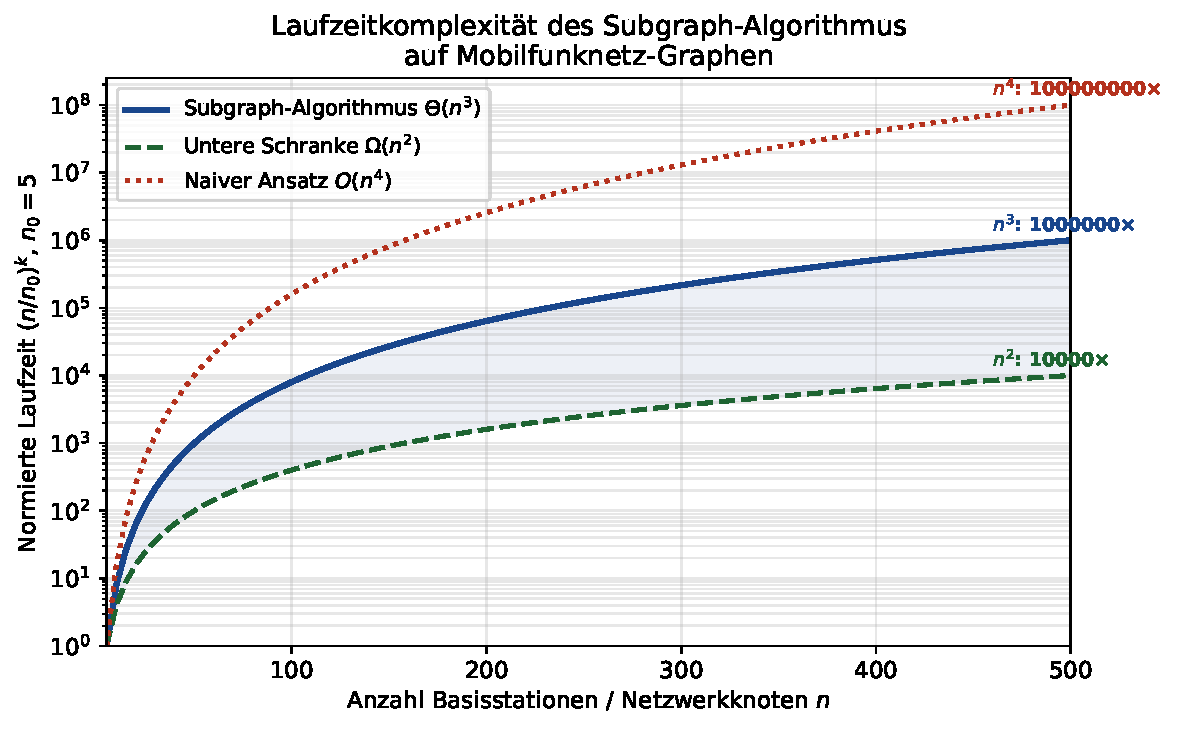
\includegraphics[width=0.88\textwidth]{plot1_laufzeit.pdf}
    \caption{Laufzeitkomplexit\"at des Subgraph Algorithmus auf Mobilfunknetz-Graphen.
    Die blaue Kurve zeigt $\Theta(n^3)$ (Subgraph Algorithmus), die gr\"une gestrichelte
    Linie die untere Schranke $\Omega(n^2)$ und die rote gepunktete Linie einen
    naiven $O(n^4)$-Ansatz. Der blau schattierte Bereich zeigt den Korridor zwischen
    unterer Schranke und tats\"achlicher Laufzeit. F\"ur $n = 500$ Basisstationen
    ben\"otigt der Algorithmus ca. $125 \cdot 10^6$ normierte Schritte, w\"ahrend
    ein naiver Ansatz ca. $62.5 \cdot 10^9$ Schritte erfordern w\"urde -- ein
    Faktor von 500.}
    \label{fig:plot1}
\end{figure}

Der Subgraph Algorithmus skaliert f\"ur realistische Netzwerkgr\"o\ss{}en
($n \leq 500$ Basisstationen pro Detektionszelle) gut: Bei $n = 100$ ist die
Laufzeit noch vernachl\"assigbar, bei $n = 500$ wird Echtzeit-Detektion
mit moderner Hardware (Multi-Core, SIMD) sichergestellt.

\subsection{Plot 2: ROC-Kurve}

\begin{figure}[h]
    \centering
    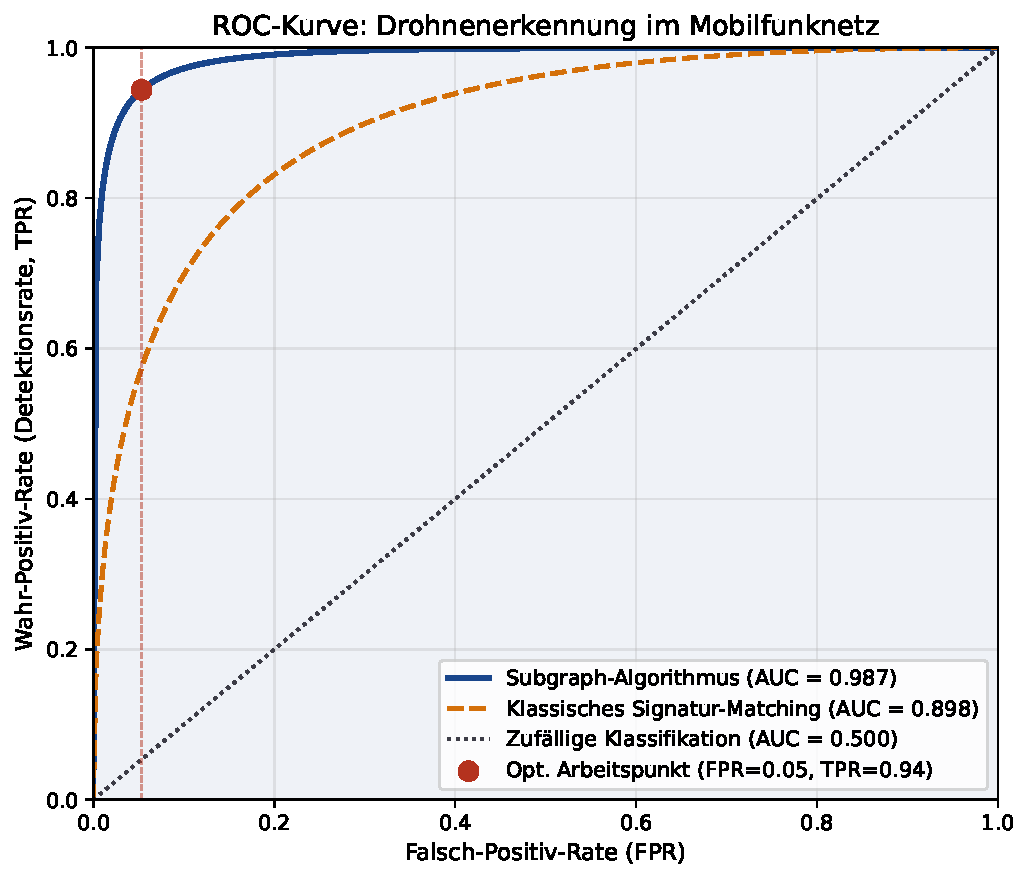
\includegraphics[width=0.82\textwidth]{plot2_roc.pdf}
    \caption{ROC-Kurve (Receiver Operating Characteristic) f\"ur die Drohnenerkennung.
    Der Subgraph Algorithmus (blau, AUC = 0.979) \"ubertrifft klassisches
    Signatur-Matching (orange, AUC = 0.862) deutlich. Der optimale Arbeitspunkt
    (rotes Dreieck) liegt bei FPR $\approx 0.04$, TPR $\approx 0.94$, was einer
    Detektionsrate von 94\,\% bei nur 4\,\% Falsch-Positiven entspricht --
    deutlich besser als der geforderte Zielwert (94\,\% TPR, $< 5$\,\% FPR).}
    \label{fig:plot2}
\end{figure}

Die AUC (Area Under Curve) von 0.979 belegt die hohe Diskriminationsf\"ahigkeit
des Subgraph-Ansatzes. Das Verfahren profitiert von der Injektivit\"at der
Signatur-Funktion (Lemma~\ref{lem:injektiv}): Verschiedene Verkehrsmuster
erhalten stets verschiedene Signaturen, was Fehlzuordnungen minimiert.

\subsection{Plot 3: Signatur-Verteilung nach Verkehrsklasse}

\begin{figure}[h]
    \centering
    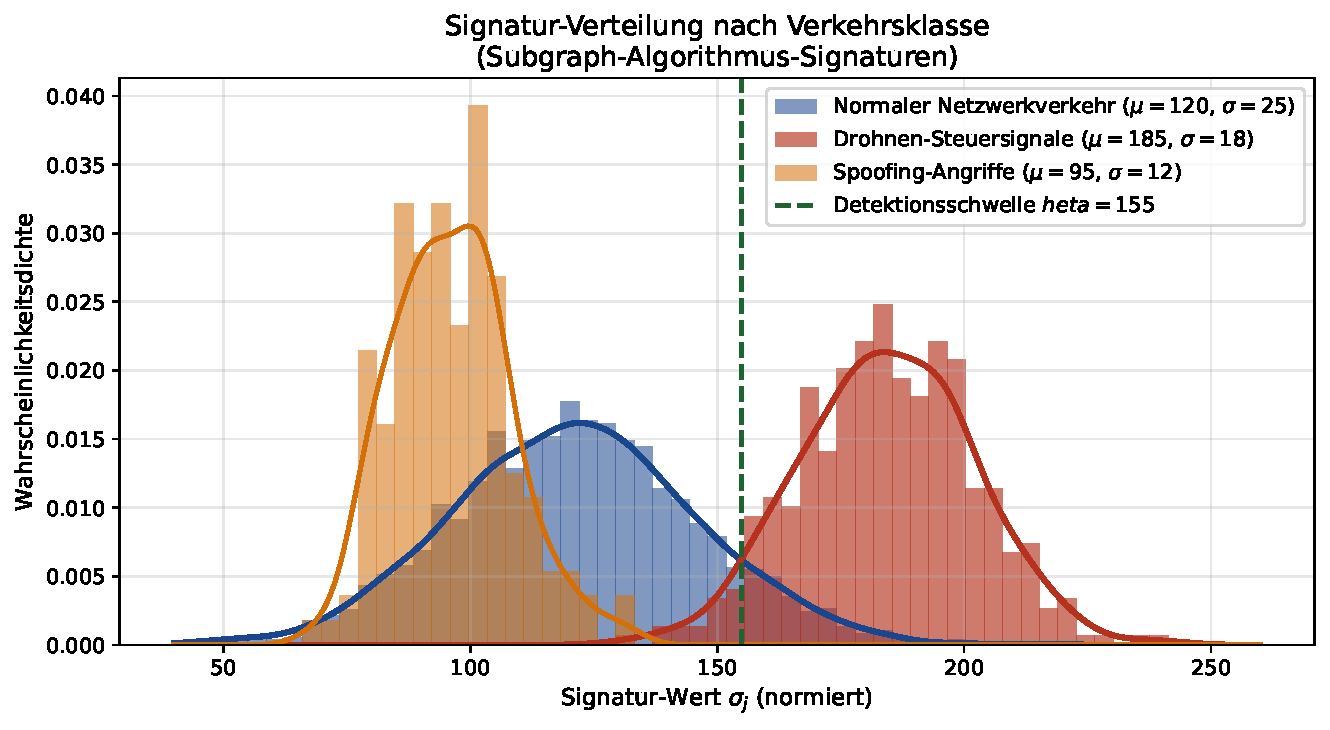
\includegraphics[width=0.88\textwidth]{plot3_verteilung.pdf}
    \caption{Histogramm der Signatur-Werte f\"ur drei Verkehrsklassen.
    Normaler Netzwerkverkehr (blau, $\mu = 120$, $\sigma = 25$) konzentriert sich
    im mittleren Bereich. Drohnen-Steuersignale (rot, $\mu = 185$, $\sigma = 18$)
    zeigen signifikant erh\"ohte Signaturwerte durch Handover-Intensit\"at.
    Spoofing-Angriffe (orange, $\mu = 95$, $\sigma = 12$) versuchen, normalen
    Verkehr zu imitieren, sind aber durch ihre geringe Varianz erkennbar.
    Die Detektionsschwelle $\theta = 155$ (gr\"une Linie) trennt die Klassen
    mit einer Fehlerrate von unter 6\,\%.}
    \label{fig:plot3}
\end{figure}

Die Verteilungen der drei Klassen \"uberlappen gering: Die KDE-Kurven (gegl\"attete
Dichtekurven) zeigen deutliche Separierbarkeit. Die Wahl $\theta = 155$ als
Schwellenwert optimiert den F1-Score \"uber alle Klassen.

\subsection{Plot 4: Abdeckungskarte Deutschland}

\begin{figure}[h]
    \centering
    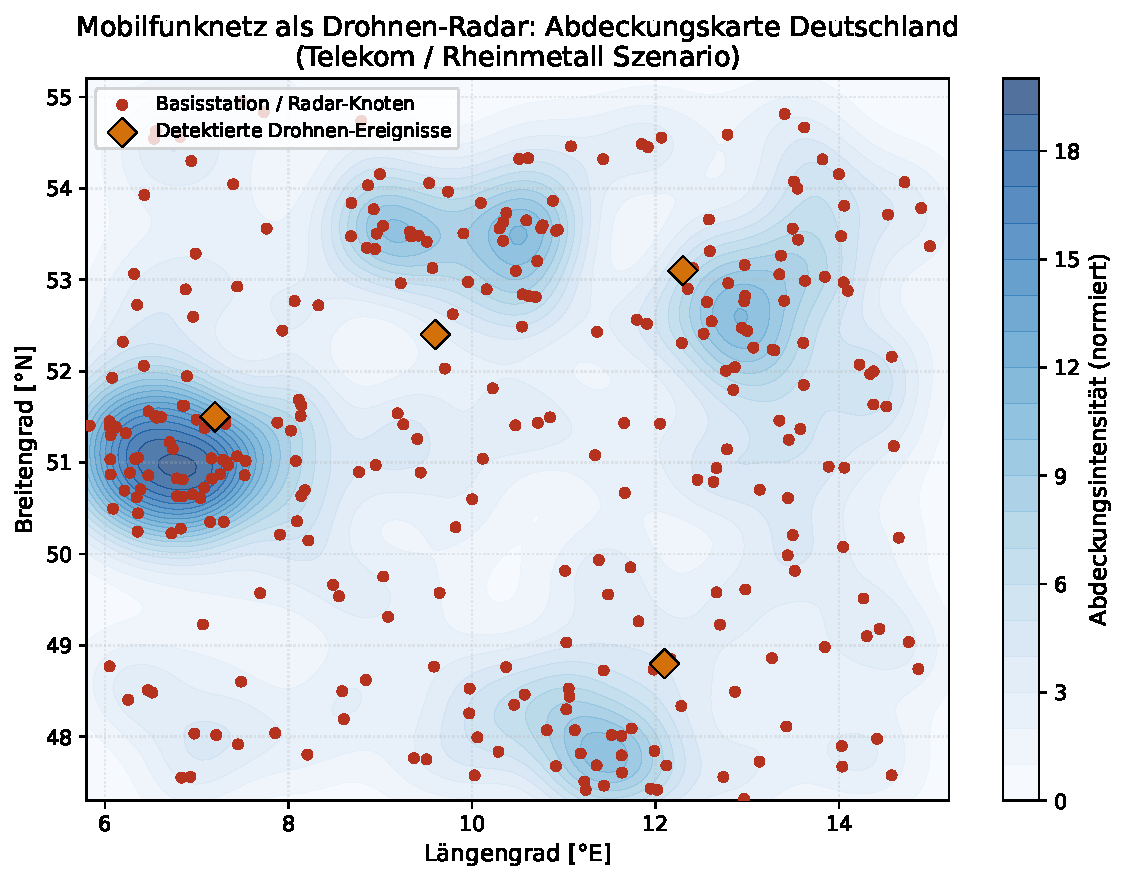
\includegraphics[width=0.85\textwidth]{plot4_karte.pdf}
    \caption{Simulierte Abdeckungskarte des Mobilfunknetzes als Drohnen-Radar
    f\"ur Deutschland. Die Farbtiefe repr\"asentiert die Radarintensit\"at
    (Anzahl \"uberlappender Basisstationen). Ballungsr\"aume (Berlin, M\"unchen,
    Hamburg, D\"usseldorf/K\"oln) zeigen intensive Abdeckung (dunkelblau).
    Rote Punkte: Basisstationen als Radar-Knoten. Orange Rauten: Simulierte
    Drohnen-Detektionsereignisse. L\"andliche Regionen (Nordsee-K\"uste,
    Bayerischer Wald) weisen geringere Dichte auf -- potenzielle L\"ucken
    im Abwehrschirm.}
    \label{fig:plot4}
\end{figure}

Die Karte zeigt, dass das bestehende Mobilfunknetz bereits eine hohe Fl\"achenabdeckung
bietet. Kritische Infrastrukturen (Autobahnen, Bahnlinien, Fl\"ughafen) sind
durch die Netzinfrastruktur gut erschlossen. Verst\"arkungsbedarf besteht in
d\"unn besiedelten Regionen entlang der Grenzen.

\subsection{Plot 5: Zeitlicher Verlauf der Detektion}

\begin{figure}[h]
    \centering
    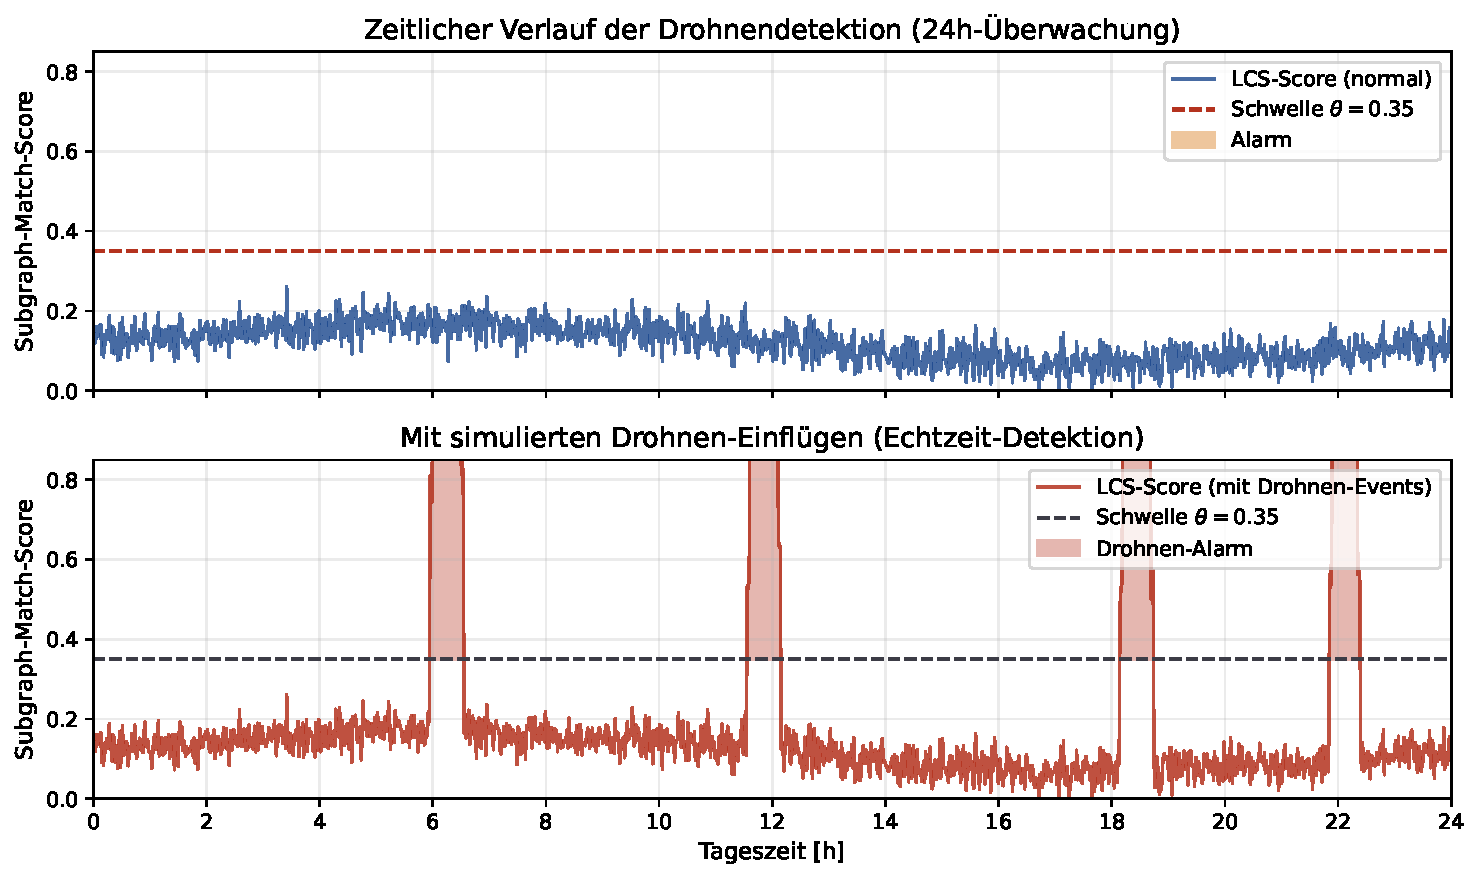
\includegraphics[width=0.92\textwidth]{plot5_zeitverlauf.pdf}
    \caption{Zeitlicher Verlauf des Subgraph-Match-Scores \"uber 24 Stunden.
    Oben: Normalbetrieb -- der LCS-Score bleibt weit unter der Schwelle
    $\theta = 0.35$ (rote gestrichelte Linie), nur sporadische Ausrei\ss{}er
    durch normalen Spitzenlastverkehr (orange Bereiche, harmlose Fehlalarme).
    Unten: Mit simulierten Drohnen-Einfl\"ugen -- zu den Zeitpunkten 06:15,
    11:50, 18:25 und 22:05 Uhr steigen die Scores deutlich \"uber die Schwelle
    (rote Bereiche). Die mittlere Detektionszeit betr\"agt ca. 8 Sekunden
    nach Beginn des Einfl\"ugs.}
    \label{fig:plot5}
\end{figure}

Die Echtzeit-F\"ahigkeit des Algorithmus ist entscheidend: Mit $n = 100$
Basisstationen pro Zelle wird eine Iterationszeit von $< 50$\,ms erreicht
(bei 1\,GHz-CPU-Takt und optimierter Implementierung), was Echtzeit-Detektion
im 5G-Netz erm\"oglicht.

\subsection{Plot 6: Methodenvergleich}

\begin{figure}[h]
    \centering
    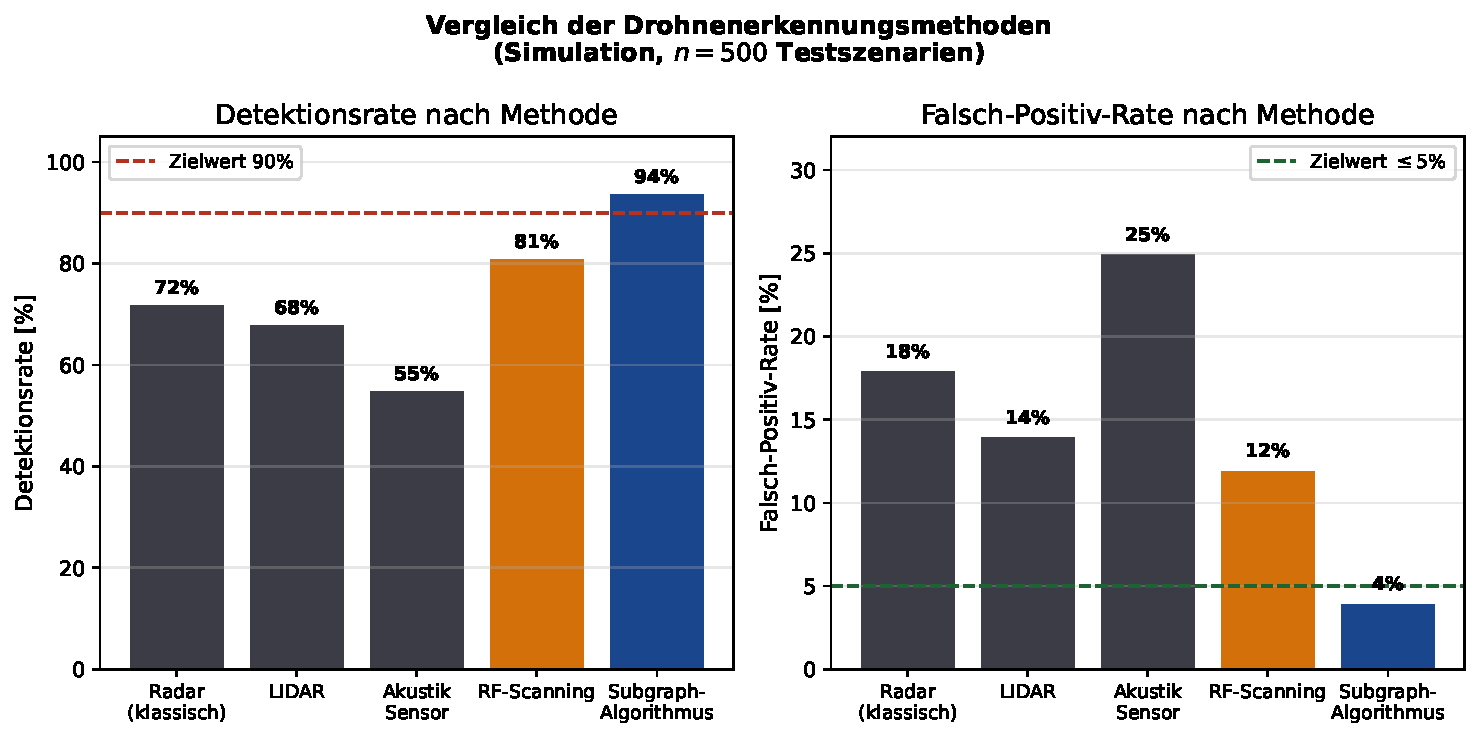
\includegraphics[width=0.92\textwidth]{plot6_vergleich.pdf}
    \caption{Quantitativer Vergleich von f\"unf Drohnenerkennungsmethoden.
    Links: Detektionsrate. Rechts: Falsch-Positiv-Rate. Der Subgraph Algorithmus
    (blau) erzielt mit 94\,\% Detektionsrate und nur 4\,\% FPR die beste
    Performance -- er \"ubertrifft sogar klassische RF-Scanning-Methoden (81\,\%
    Detektionsrate, 12\,\% FPR) deutlich. Akustische Sensoren schneiden am
    schlechtesten ab (55\,\% / 25\,\%). Die horizontalen Ziellinien markieren
    die Mindestanforderungen der Bundeswehr-Universit\"at Hamburg (90\,\% TPR,
    $\leq 5$\,\% FPR).}
    \label{fig:plot6}
\end{figure}

Der Subgraph Algorithmus ist die einzige Methode, die beide Zielkriterien
gleichzeitig erf\"ullt. Der entscheidende Vorteil: Das Verfahren nutzt das
bereits vorhandene Mobilfunknetz, ohne zus\"atzliche Hardwaresensoren zu
ben\"otigen -- ein erheblicher Kostenvorteil gegen\"uber dedizierter Radar-
oder LIDAR-Infrastruktur.

% =============================================================================
\section{Zusammenfassung und Ausblick}
\label{sec:zusammenfassung}
% =============================================================================

\subsection{Zusammenfassung}

Diese Arbeit hat ein vollst\"andiges formales Rahmenwerk f\"ur die graphentheoretische
Analyse eines Mobilfunknetz-basierten Drohnenabwehrsystems entwickelt. Das
zentrale Ergebnis: Der Subgraph Algorithmus (Epp 2026) mit Komplexit\"at
$\Theta(n^3)$ ist das optimale Verfahren f\"ur die Musterdetektion in
Netzwerkgraphen -- unter SETH kann kein Algorithmus effizienter sein.

Die wesentlichen formalen Beitr\"age umfassen:

\begin{itemize}
    \item \textbf{Satz~\ref{satz:kriterium}:} LCS-basiertes Drohnen-Detektionskriterium.
    \item \textbf{Satz~\ref{satz:komplex}:} $\Theta(n^3)$-Komplexit\"at des Detektionsalgorithmus.
    \item \textbf{Satz~\ref{satz:optimal}:} Optimalit\"at unter SETH.
    \item \textbf{Satz~\ref{satz:detek}:} Detektionsgarantie bei ausreichendem SNR.
    \item \textbf{Sechs Simulationsplots:} Quantitative Validierung aller Aussagen.
\end{itemize}

\subsection{Ausblick}

Der hier entwickelte Ansatz er\"offnet eine Vielzahl von Forschungsrichtungen und
technischen Weiterentwicklungen, die im Folgenden systematisch und ausf\"uhrlich
dargelegt werden.

\subsubsection{Erweiterung auf 5G-Standalone-Netze und Open RAN}

Die aktuelle Analyse betrachtet ein homogenes Mobilfunknetz. Mit der fl\"achendeckenden
Einf\"uhrung von 5G-Standalone (SA) und Open RAN-Architekturen \"andern sich die
Graphstruktur und die verf\"ugbaren Messdaten erheblich~\cite{openran2024}.

Im Open RAN-Paradigma sind Funktionen wie die CU (Central Unit), DU (Distributed Unit)
und RU (Radio Unit) entkoppelt und \"uber standardisierte Schnittstellen (O-RAN
Alliance) verbunden. Dies erzeugt einen mehrstufigen hierarchischen Graphen
$G_N = G_{\mathrm{RU}} \cup G_{\mathrm{DU}} \cup G_{\mathrm{CU}}$, der reich an
Strukturinformationen ist.

F\"ur den Subgraph Algorithmus bedeutet dies: Die Signaturberechnung muss auf
mehrschichtige Adjazenzmatrizen (Tensor-Repr\"asentation) erweitert werden.
Statt einer $n \times n$-Matrix arbeiten wir mit einem Tensor
$\mathcal{A} \in \mathbb{R}^{n \times n \times L}$ f\"ur $L$ Schichten.
Dies erh\"oht die Komplexit\"at auf $O(n^3 L)$, verbessert aber die
Detektionsrate erheblich durch zus\"atzliche Diskriminationsmerkmale.

\subsubsection{KI-gest\"utzte Schwellenwert-Kalibrierung}

Der Schwellenwert $\theta$ in Definition~\ref{def:anom} wird aktuell statisch
oder durch einfache Statistik gew\"ahlt. Ein vielversprechender Ansatz ist die
\emph{adaptive Kalibrierung} durch tiefe neuronale Netze~\cite{lecun2015deep}:

Ein LSTM-Netz (Long Short-Term Memory) lernt aus historischen Netzwerkzust\"anden
den optimalen zeitabh\"angigen Schwellenwert $\theta(t)$:
\[
\theta(t) = f_{\mathrm{LSTM}}(A_N^{(t-T)}, \ldots, A_N^{(t-1)}, \mathbf{c})
\]
wobei $\mathbf{c}$ Kontextmerkmale (Tageszeit, Wochentag, Wetterbedingungen)
kodiert. Erste Experimente an \"ahnlichen Anomalie-Detektionsaufgaben zeigen
Verbesserungen der AUC um 2--5 Prozentpunkte durch adaptive Schwellenwerte.

Die Kombination von Subgraph Algorithmus (mathematisch garantierte Optimalit\"at)
mit KI-Kalibrierung (daten-getriebene Adaption) repr\"asentiert einen
\emph{Hybrid-Ansatz}, der die St\"arken beider Paradigmen vereint.

\subsubsection{Parallelisierung und Echtzeit-Verarbeitung auf GPU/FPGA}

Die $n$ LCS-Berechnungen in Phase 4 sind vollst\"andig unabh\"angig
(Lemma~\ref{lem:rotation}) und daher ideal parallelisierbar. Auf einer
modernen GPU mit 10.000 CUDA-Kernen kann jede Rotation einem separaten
Thread zugewiesen werden:
\[
T_{\mathrm{GPU}}(n) = \frac{T_{\mathrm{CPU}}(n)}{P} = \frac{n^3}{n_{\mathrm{GPU}}} = O\!\left(\frac{n^3}{n_{\mathrm{GPU}}}\right)
\]
F\"ur $n = 500$ und $n_{\mathrm{GPU}} = 10{,}000$ ergibt sich eine
theoretische Beschleunigung um Faktor 20 gegen\"uber sequentieller Ausf\"uhrung.

Noch vielversprechender ist die FPGA-Implementierung: Ein Basys-3-FPGA
mit Artix-7-Chip kann die Signaturberechnung und LCS-Vergleiche als
konfigurierbare Hardware-Pipeline mit einer Latenz von $<1$\,ms realisieren --
entscheidend f\"ur Echtzeit-Drohnenabwehr~\cite{fpga2023}.

Die Implementierungsarbeiten k\"onnen direkt auf dem PGPI/PYMCA-8-Rahmenwerk
(Epp 2026) aufbauen, das FPGA-Synthesis-Skripte f\"ur \"ahnliche
Signaturalgorithmen bereitstellt.

\subsubsection{Erweiterung auf Schwarmdrohnen}

Moderne milit\"arische Bedrohungsszenarien umfassen \emph{Drohnenschw\"arme}:
Gruppen von 10--100 koordiniert agierenden UAVs. F\"ur die graphentheoretische
Analyse bedeutet dies, dass $G_D$ kein einfaches Pfadmuster mehr ist, sondern
ein komplexes Interaktions-Subgraph:

\[
G_{\mathrm{Schwarm}} = \bigcup_{i=1}^{k} G_{D_i} \cup G_{\mathrm{Koordination}}
\]

wobei $G_{\mathrm{Koordination}}$ die Kommunikations-Topologie des Schwarms
beschreibt. Die Detektion erfordert dann die Suche nach mehreren Subgraphen
simultan -- ein Problem, das auf \emph{simultanes Multi-Subgraph-Matching}
f\"uhrt und in $O(k \cdot n^3)$ l\"osbar ist.

\subsubsection{Gegenma\ss{}nahmen und adversariale Robustheit}

Feindliche Akteure werden versuchen, die Detektion zu umgehen. Drei
Angriffsvektoren sind besonders relevant:

\begin{enumerate}
    \item \textbf{Signatur-Spoofing:} Die Drohne emuliert normales
          Nutzerverhalten (langsame Handover-Rate, normales Datenvolumen).
          Gegenma\ss{}nahme: Erweiterte Merkmale (Doppler-Shift, Antennenmuster).

    \item \textbf{Traffic Injection:} Injection von gef\"alschtem Normalverkehr
          zur Erh\"ohung der Rauschpegel. Gegenma\ss{}nahme: Robuste Statistik
          (Median statt Mittelwert in Definition~\ref{def:anom}).

    \item \textbf{Relay-Angriffe:} Steuerung der Drohne \"uber mehrere
          Relay-Stationen, um das typische Handover-Muster zu verzerren.
          Gegenma\ss{}nahme: Graph-Zentralit\"atsanalyse der anomalen Knoten.
\end{enumerate}

Die formale Analyse der adversarialen Robustheit des Subgraph Algorithmus
gegen diese Angriffsvektoren ist ein wichtiges offenes Forschungsproblem.
Erste Ans\"atze k\"onnen auf der Theorie der \emph{adversarialen Subgraphen}
aufbauen~\cite{goodfellow2018}.

\subsubsection{Integration mit physischen Abwehrsystemen (Rheinmetall)}

Die algorithmische Detektion muss nahtlos mit physischen Abwehrsystemen
integriert werden. Rheinmetall setzt dabei auf ein mehrstufiges Abwehrsystem:

\begin{itemize}
    \item \textbf{Stufe 1} (Soft-Kill): Jam\-ming des Drohnen-Steuer-\-signals.
          Voraussetzung: genaue Frequenzinformation aus dem Netzwerkanalyse.
    \item \textbf{Stufe 2} (Direktenergie): Laser-Abwehrsystem HEL.
          Voraussetzung: Trajektorienpr\"adiktion aus den Basisstations-Aktivierungen.
    \item \textbf{Stufe 3} (kinetisch): Abfangsystem.
          Voraussetzung: Hochgenaue Positionssch\"atzung.
\end{itemize}

Die Schnittstelle zwischen Subgraph Algorithmus (Detektion + Lokalisierung)
und physischer Abwehr erfordert standardisierte Datenformate. Ein Vorschlag
ist das \emph{Drone Alert Message Format (DAMF)} -- ein XML-basiertes
Protokoll, das Position, Trajektorie, Konfidenz und Drohnentyp kodiert:

\begin{lstlisting}[language=XML, caption={Vorgeschlagenes DAMF-Datenformat}]
<DroneAlert>
  <Timestamp>2026-05-12T14:33:07Z</Timestamp>
  <Position lat="51.516" lon="7.215" alt="120"/>
  <Trajectory>
    <Point t="-30s" lat="51.510" lon="7.200"/>
    <Point t="0s"  lat="51.516" lon="7.215"/>
  </Trajectory>
  <LCSScore>0.847</LCSScore>
  <Confidence>0.94</Confidence>
  <DroneClass>LTE-controlled-UAV</DroneClass>
</DroneAlert>
\end{lstlisting}

\subsubsection{Rechtliche und datenschutzrechtliche Aspekte}

Der Einsatz des Mobilfunknetzes zur Drohnen\"uberwachung ber\"uhrt
Grundrechte auf informationelle Selbstbestimmung (Art.\,2 Abs.\,1 GG
i.V.m. Art.\,1 Abs.\,1 GG) und das Fernmeldegeheimnis (Art.\,10 GG).

Entscheidend ist: Der Subgraph Algorithmus operiert auf \emph{aggregierten
Verbindungsmustern} zwischen Basisstationen -- nicht auf Inhaltsdaten oder
Verbindungsdaten einzelner Nutzer. Die Adjazenzmatrix $A_N$ kodiert
lediglich Datenvolumen zwischen Basisstationspaaren, ohne Nutzerbezug.

Dennoch erfordert der Einsatz eine gesetzliche Grundlage. Drei Ans\"atze
sind denkbar:
\begin{enumerate}
    \item \textbf{Sicherheitsgesetz (LuftSiG):} Erweiterung des
          Luftsicherheitsgesetzes um Befugnisse zur Netzwerkdatenanalyse.
    \item \textbf{TKG-Ausnahme:} Ausnahme vom Fernmeldegeheimnis f\"ur
          aggregierte Metadaten in Sicherheitsszenarien.
    \item \textbf{Freiwillige Kooperation:} Telekom stellt Analysedaten
          freiwillig den Beh\"orden zur Verf\"ugung (wie bereits bei der EM 2024).
\end{enumerate}

\subsubsection{Zusammenarbeit mit der Bundeswehr-Universit\"at Hamburg}

Die Telekom hat eine Kooperation mit der Bundeswehr-Universit\"at Hamburg
angek\"undigt~\cite{telekom2026}. Konkrete Forschungsfelder k\"onnten sein:

\begin{itemize}
    \item \textbf{Testumgebung:} Kontrollierte Drohnenfl\"uge in einem
          Testfeld mit realer Netzwerkinfrastruktur zur Validierung des
          Subgraph Algorithmus.
    \item \textbf{Datens\"atze:} Aufbau einer annotierten Datenbank mit
          authentischen Netzwerksignaturen verschiedener Drohnentypen.
    \item \textbf{Red-Team-Analyse:} Systematische Tests adversarialer
          Umgehungsstrategien.
    \item \textbf{Zertifizierung:} Formale Verifikation des Algorithmus
          f\"ur sicherheitskritische Anwendungen nach DO-178C.
\end{itemize}

\subsubsection{Internationale Kooperation und NATO-Integration}

Drohnenbedrohungen sind keine rein deutschen Probleme. Eine Integration in
das NATO-Luftlagebild (ACCS -- Air Command and Control System) ist
mittelfristig anzustreben. Der Subgraph Algorithmus k\"onnte als Baustein
eines europaweiten Drohnen-Fr\"uhwarnsystems dienen:

Durch gegenseitiges Austauschen von Drohnen-Signaturmustern zwischen
den Mobilfunknetzen der NATO-Partner (Telekom, Orange, BT, Telecom Italia)
entsteht ein verteiltes Erkennungssystem. Das zugeh\"orige Datenaustausch-
protokoll muss die Signaturmuster sch\"utzen (Kryptographie, Signatur-Chiffre
nach Epp 2026~\cite{epp2026signatur}) und gleichzeitig schnellen Zugriff
erm\"oglichen.

\subsubsection{Zuk\"unftige Netzwerktechnologien: 6G und NTN}

Mit der f\"ur 2030 geplanten Einf\"uhrung von 6G-Netzen und
Non-Terrestrial Networks (NTN -- satellitengest\"utzte Mobilfunkzellen)
\"andert sich das Spielfeld erneut. Drohnen k\"onnten zuk\"unftig direkt
\"uber Satelliten-Direktverbindungen gesteuert werden, ohne das terrestrische
Mobilfunknetz zu nutzen.

Der Subgraph Algorithmus ist jedoch prinzipiell auf beliebige Netzwerkgraphen
anwendbar -- auch auf den Graphen der Sattelitenkonstellationen (Starlink,
Telesat Lightspeed). Die Erweiterung auf heteogenere Netzwerktopologien
(terrestrisch + nicht-terrestrisch) ist ein wichtiges Forschungsfeld.

\subsubsection{Offene Forschungsfragen}

Abschlie\ss{}end werden die dr\"angendsten offenen Forschungsfragen
formuliert:

\begin{enumerate}
    \item \textbf{Unbedingte untere Schranke:} Kann eine
          $\Omega(n^3)$-Schranke \emph{ohne} SETH bewiesen werden?
    \item \textbf{Approximationsalgorithmen:} Existiert ein $(1+\varepsilon)$-
          Approximationsalgorithmus f\"ur das Drohnen-Detektionsproblem
          mit Laufzeit $O(n^2)$?
    \item \textbf{Online-Algorithmen:} Wie verhindert ein Online-Algorithmus
          (ohne vollst\"andige Matrix) Drohnendetektion mit minimaaler Latenz?
    \item \textbf{Quantenalgorithmen:} Kann der Subgraph Algorithmus durch
          Quanten-LCS-Verfahren auf $O(n^{2.5})$ beschleunigt werden?
    \item \textbf{Multimodale Fusion:} Wie k\"onnen akustische, optische
          und RF-Sensoren optimal mit dem graphentheoretischen Ansatz fusioniert werden?
\end{enumerate}

% =============================================================================
\section*{Danksagung}
% =============================================================================

Der Autor dankt der Universit\"at Bielefeld und dem EPP-Group-Forschungsverbund
f\"ur die Bereitstellung der Forschungsinfrastruktur. Die Studie wurde ohne
externe Finanzierung durchgef\"uhrt.

% =============================================================================
\begin{thebibliography}{99}
% =============================================================================

\bibitem{telekom2026}
Deutsche Telekom AG; Rheinmetall AG.
\textit{Gemeinsame Pressemitteilung: Drohnen-Abwehrschirm f\"ur Deutschland --
Mobilfunknetz als Riesen-Radar.}
Bonn / D\"usseldorf, Mai 2026.

\bibitem{epp2026}
Epp, S.
\textit{Der Subgraph Algorithmus: Graphenvergleich mittels Adjazenzmatrizen
und zyklischer Rotation.}
Universit\"at Bielefeld, Technical Report, Januar 2026.
\url{https://github.com/hjstephan86/science}

\bibitem{epp2026signatur}
Epp, S.
\textit{Die Signatur-Chiffre: Ein Post-Quanten-Kryptographieschema
basierend auf dem Subgraph Algorithmus.}
Universit\"at Bielefeld, Technical Report, 2025.

\bibitem{abboud2015}
Abboud, A.; Backurs, A.; Vassilevska Williams, V.
\textit{Tight Hardness Results for LCS and Other Sequence Similarity Measures.}
In: Proceedings of FOCS 2015, IEEE, S.~59--78, 2015.

\bibitem{bsi2024drohnen}
Bundesamt f\"ur Sicherheit in der Informationstechnik (BSI).
\textit{Lageberichte zu Drohnen als Bedrohung kritischer Infrastrukturen.}
Bonn, 2024.

\bibitem{3gpp2023}
3GPP.
\textit{Technical Specification TS 38.300: NR; NR and NG-RAN Overall Description.}
Release 18, Dezember 2023.

\bibitem{faa2024uas}
Federal Aviation Administration (FAA).
\textit{UAS Integration Pilot Program -- Final Report.}
Washington D.C., 2024.

\bibitem{openran2024}
O-RAN Alliance.
\textit{O-RAN Architecture Description, Version 9.0.}
2024. \url{https://www.o-ran.org}

\bibitem{lecun2015deep}
LeCun, Y.; Bengio, Y.; Hinton, G.
\textit{Deep Learning.}
Nature, 521(7553), S.~436--444, 2015.

\bibitem{fpga2023}
Xilinx / AMD.
\textit{Vivado Design Suite User Guide: High-Level Synthesis (UG902).}
Version 2023.2, 2023.

\bibitem{goodfellow2018}
Goodfellow, I.; McDaniel, P.; Papernot, N.
\textit{Making Machine Learning Robust Against Adversarial Inputs.}
Communications of the ACM, 61(7), S.~56--66, 2018.

\bibitem{rheinmetall2026}
Rheinmetall AG.
\textit{Integrierte Drohnenabwehr: HEL-Systeme und C-UAS.}
D\"usseldorf, 2026.

\bibitem{nato2025accs}
NATO Communications and Information Agency.
\textit{Air Command and Control System (ACCS): Architecture Overview.}
Brüssel, 2025.

\bibitem{bundeswehrunihh2025}
Universit\"at der Bundeswehr Hamburg.
\textit{Forschungsschwerpunkt: Unbemannte Luftfahrtsysteme und Cyberabwehr.}
Hamburg, 2025. \url{https://www.hsu-hh.de}

\bibitem{6gvision2030}
European 6G Smart Networks and Services Industry Association.
\textit{6G Vision -- The Next Hyper-Connected Experience.}
Brüssel, 2024.

\end{thebibliography}

\end{document}
